\chapter{Development of a Web Application Programming Interface for Genome 
Properties Data} \label{micromeda-server}

As discussed in Chapter \ref{introduction}, one of the goals of Micromeda is to 
provide users with an interface for visualizing the presence and absence of 
genome properties across multiple organisms. The Micromeda software is accessed 
through a web application that uses in-file data to generate interactive heat 
map visualizations. The use of a web application has several advantages and 
these are discussed in Chapter \ref{micromeda-client}. This client application 
is supported by a web server process that parses Micromeda files and provides a 
web \gls{api} for accessing their contents. This chapter will discuss the server 
component, called Micromeda-Server, including the services it provides and its 
implementation. The client web application that uses these services is discussed 
in Chapter \ref{micromeda-client}.

\section{Overview of Web Servers} \label{web-servers}

The World Wide Web and associated web applications are ideal delivery mechanisms 
for data analysis software such as Micromeda \cite{berners1994world}. Such 
applications follow a client-server architecture \cite{svobodova1985client} (see 
\href{http://en.wikipedia.org/wiki/Client-server_model}{en.wikipedia.org/wiki/Client-server\_model}) 
where the code running in the user's browser is called the client. The user 
acquires this client by downloading it into their browser like any other 
webpage. If this client requires external data, it can request this information 
from a server process running on a server computer system\footnote{For this 
document, the term \textbf{server computer system} is used to refer to the 
physical hardware on which software is running. The term \textbf{server} is used 
to refer to a software process that provides users or applications with data.}. 
Requests to the server are made, via \gls{http} \cite{fielding1999hypertext}, 
using a series of \gls{url} addresses \cite{berners1994rfc} (\textit{i}.\textit{e}., web 
addresses) that return specific types of data. These addresses are known as 
\textbf{endpoints} (Section \ref{endpoints}) and form a web \gls{api}.

\section{Micromeda-Server Workflow and Implementation} \label{server-workflow}

\begin{figure}[!ht]
  \centering
	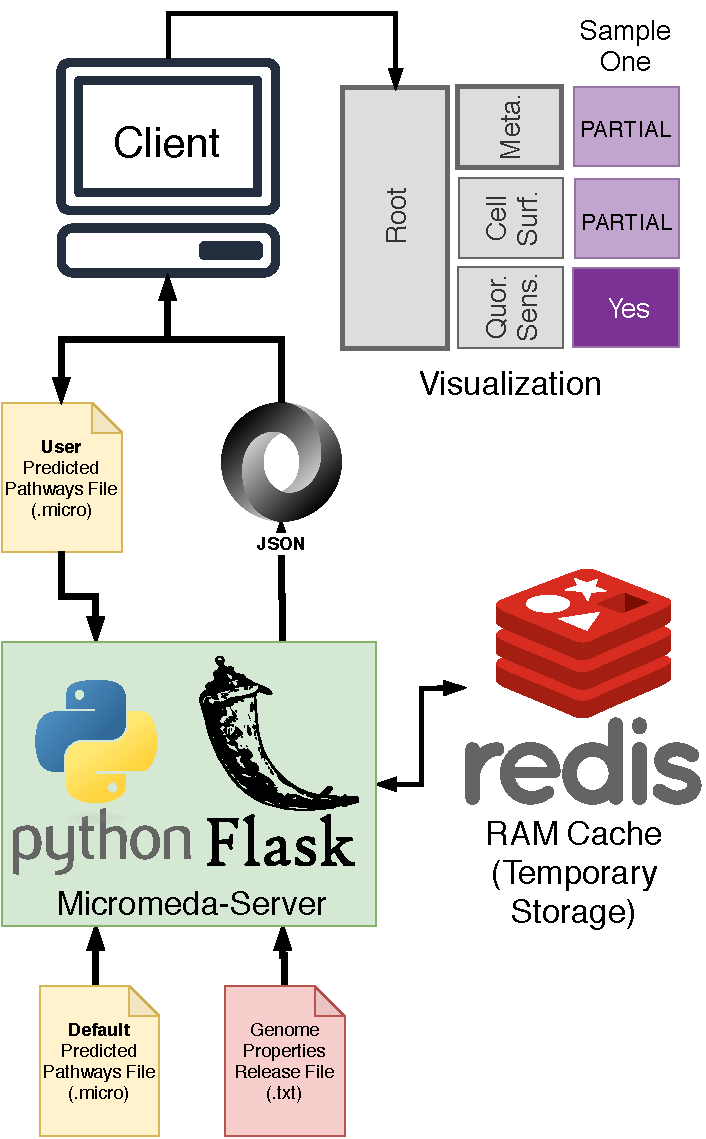
\includegraphics[width=0.50\textwidth]{media/Micromeda-Server.pdf}
	 \caption[Micromeda-Server is a web server application consisting of several 
components.]{\textbf{Micromeda-Server is a web server application consisting of 
several components.} The server code was written in Python using the Flask web 
framework \cite{grinberg2018flask}. Micromeda-Server is supported by a Redis 
cache and a series of text files. A genomeproperties.txt file supplies data for 
the generation of Genome Properties \gls{dag}. Micromeda files, either default 
or uploaded, provide information about property assignments, step assignments, 
and supporting information of multiple organisms.}
	 \label{fig:micromeda-server}
\end{figure}

\begin{figure}[!ht]
  \centering
	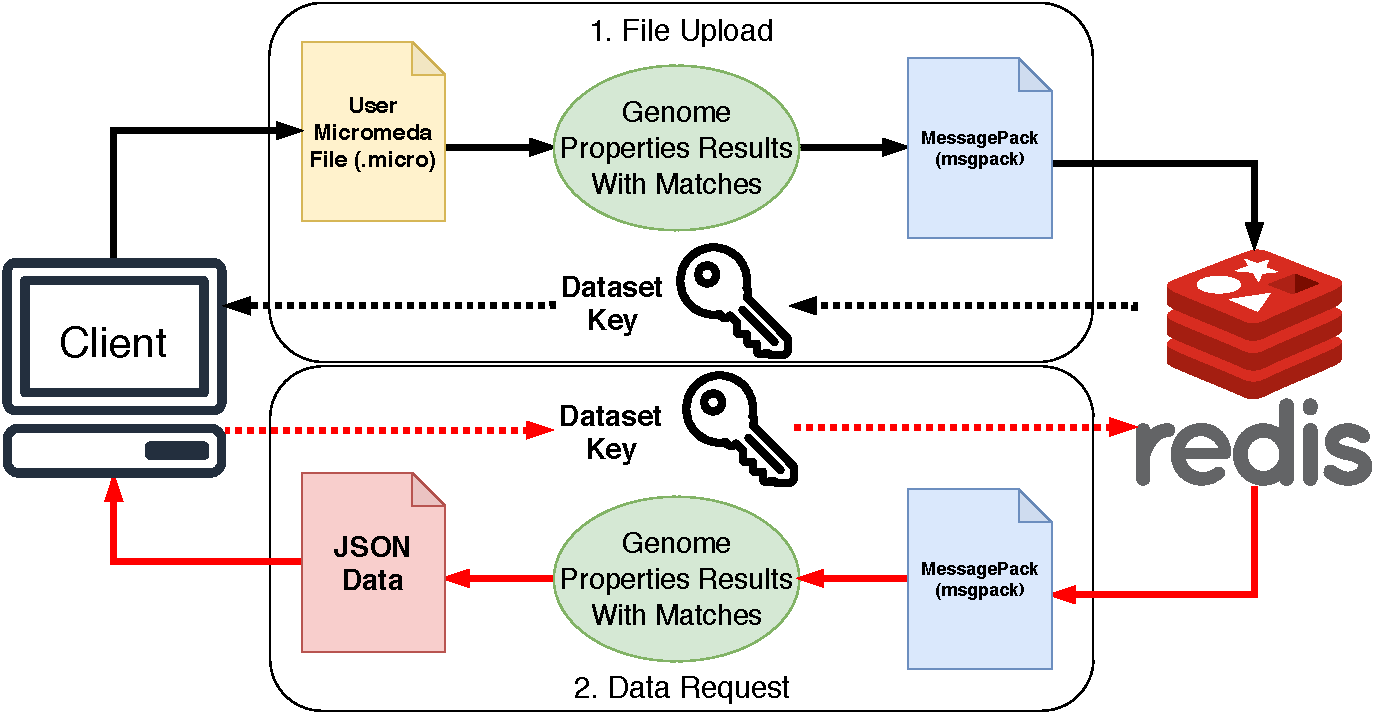
\includegraphics[width=0.80\textwidth]{media/Micromeda-Server-Workflow.pdf}
	 \caption[Once a Micromeda file is uploaded, Micromeda-Server caches its 
contents in Redis.]{\textbf{Once a Micromeda file is uploaded, Micromeda-Server 
caches its contents in Redis.} The caching process involves the generation of 
GenomePropertiesResultsWithMatches objects for each uploaded file. These objects 
are cached in Redis and reconstituted between API calls. Micromeda-Server uses 
methods possessed by these reconstituted GenomePropertiesResultsWithMatches 
objects to produce responses that are sent back to a web client application. 
Each uploaded file is assigned a dataset key that is provided to the client. The 
client later uses this key to request data from a specific Micromeda file.}
	 \label{fig:micromeda-server-workflow}
\end{figure}

\begin{figure}[!ht]
  \centering
	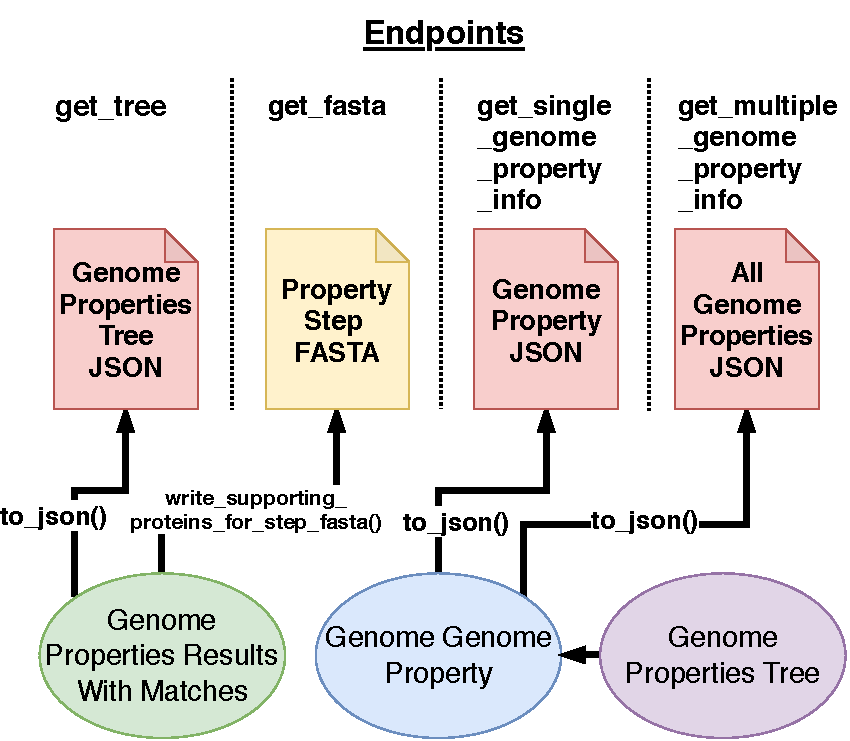
\includegraphics[width=0.65\textwidth]{media/Micromeda-Endpoints.pdf}
	 \caption[Micromeda-Server currently presents four endpoints for accessing 
Genome Properties and Micromeda file data.]{\textbf{Micromeda-Server currently 
presents four endpoints for accessing Genome Properties and Micromeda file 
data.} These endpoints return JSON documents and FASTA files that are generated 
using methods of GenomePropertiesResultsWithMatches objects, GenomeProperty 
objects, and GenomePropertiesTree objects.}
	 \label{fig:micromeda-endpoints}
\end{figure}

Micromeda-Server is designed to provide a web \gls{api} to client applications 
that require access to information about the Genome Properties database. It also 
provides an \gls{api} for accessing temporarily stored property assignments, 
step assignments, and supporting information for user-supplied datasets. The 
Micromeda-Server is written in Python and utilizes the Flask web development 
framework \cite{grinberg2018flask} (Fig. \ref{fig:micromeda-server}) to map 
Python functions for handling specific web \gls{api} requests to server 
\gls{url} addresses (\textit{i}.\textit{e}., ``endpoints"). Information about the Genome 
Properties database is supplied to Micromeda-Server via a 
\textbf{genomeProperties.txt} release file (Fig. \ref{fig:micromeda-server} and 
Subsection \ref{Genome-Properties-Files}). Property assignments, step 
assignments, and supporting information for user datasets are supplied via 
user-uploaded Micromeda files (Fig. \ref{fig:micromeda-server}). These Micromeda 
files are parsed into GenomePropertyResultsWithMatches objects (Subsection 
\ref{PropertyResultsWithMatches}) that are later stored in an in-memory Redis 
cache \cite{han2011survey} in MessagePack format \cite{furuhashi2013messagepack} 
(Fig. \ref{fig:micromeda-server}, Fig. \ref{fig:micromeda-server-workflow} and 
Section \ref{msgpack}). In the context of Micromeda-Server, the contents of each 
uploaded and cached Micromeda file is called a dataset. A single Micromeda file 
can also be provided to Micromeda-Server during start-up for use as default 
dataset (Fig. \ref{fig:micromeda-server}). This default dataset is also parsed 
to a GenomePropertiesResultsWithMatches object and is used to supply data to the 
\gls{api} if users upload no Micromeda files. The standard workflow for starting 
and then using Micromeda-Server is the following:

\begin{enumerate}
  \item Start Micromeda-Server while providing a \textbf{genomeProperties.txt} 
file and an optional default Micromeda file (Fig. \ref{fig:micromeda-server})
  \item The \textbf{genomeProperties.txt} file is parsed to a 
GenomePropertiesTree object
  \item The default dataset Micromeda file is parsed to a 
GenomePropertiesResultsWithMatches object  
  \item The client application sends a user-supplied Micromeda file to the 
server via the upload endpoint (Fig. \ref{fig:micromeda-server-workflow})
  \item The user-supplied Micromeda files are parsed to a 
GenomePropertiesResultsWithMatches object that is later stored in the Redis 
cache in MessagePack format (Fig. \ref{fig:micromeda-server-workflow})
  \item The server supplies the client with a dataset key that is unique to each 
uploaded Micromeda file (Fig. \ref{fig:micromeda-server-workflow})
  \item The client can later supply this dataset key to the server during 
proceeding \gls{api} requests to get information from the previously uploaded 
Micromeda file (Fig. \ref{fig:micromeda-server-workflow})
  \item If the client provides no dataset key then the server supplies 
information about the default dataset during \gls{api} requests
\end{enumerate}

Each GenomePropertiesResultsWithMatches object cached to Redis is given a 
\gls{ttl} value \cite{gwertzman1996world} (see 
\href{http://en.wikipedia.org/wiki/Time_to_live}{en.wikipedia.org/wiki/Time\_to\_live}). 
Users can set this value for any period, such as minutes or days. After the 
\gls{ttl} of the cached object is exceeded, it is flushed from the cache; the 
user will then have to re-upload their Micromeda file. The default \gls{ttl} 
used is two hours. During each \gls{api} request, if a dataset key is provided, 
the MessagePack-formatted GenomePropertiesResultsWithMatches object is grabbed 
from the cache and reconstituted into its original form (Fig. 
\ref{fig:micromeda-server-workflow}). During the \gls{api} call this 
reconstituted GenomePropertiesResultsWithMatches object's methods are used to 
supply data to the client  (Fig. \ref{fig:micromeda-server-workflow} and Fig. 
\ref{fig:micromeda-endpoints}). Further details on these endpoints are provided 
in Section \ref{endpoints}.

Micromeda files contain information about both assignments and supporting 
information used in their creation. This supporting information, such as 
proteins sequences, can take up substantial disk space. Permanently storing such 
information would be prohibitive in terms of both hardware and maintenance 
costs. In response, Micromeda-Server was designed to store uploaded datasets 
temporarily. Uploads to the server are done anonymously. 

\section{Use of Redis for Dataset Caching} \label{redis-caching}

Python, due to limitations in its default cPython interpreter 
\cite{van1995python}, is only capable executing one compute thread 
\cite{saltzer1966traffic} (see 
\href{http://en.wikipedia.org/wiki/Thread_(computing)}{en.wikipedia.org/wiki/Thread\_(computing)}) 
at a time \cite{beazley2010understanding}. This limitation causes problems for 
web server \gls{api}s that are required to handle multiple requests from clients 
simultaneously. In response, the majority of Python web frameworks, which 
provide boilerplate code for writing \gls{api} endpoints, are designed to run 
multiple copies of the Python code, which handles endpoint requests (Fig. 
\ref{fig:client-processing}). Flask is one such framework 
\cite{grinberg2018flask}. These codes are run in separate processes (see 
\href{http://en.wikipedia.org/wiki/Thread_(computing)\#Threads\_vs.\_processes}{en.wikipedia.org/wiki/ 
Thread\_(computing)\#Threads\_vs.\_processes}) and do not share a memory space 
(Fig. \ref{fig:client-processing}). Thus, any in-memory objects created for one 
\gls{api} request are not shared with the others (Fig. 
\ref{fig:client-processing}). Also, there is no guarantee that subsequent 
\gls{api} requests from a single web client will be mapped repeatedly to the 
same \gls{api} server process (Fig. \ref{fig:client-processing}). This lack of 
mapping causes a problem as a GenomePropertiesResultsWithMatches object created 
by an upload would be stored in only one process and would not be available to 
other processes that future client requests may call (Fig. 
\ref{fig:client-processing}). One way of circumventing this process isolation 
issue is to store data to be shared between web server processes in an external 
process that is used as a cache (Fig. \ref{fig:micromeda-server-workflow} and 
Fig. \ref{fig:client-processing}). This way, all web \gls{api} processes have 
one place where they access shared data. Micromeda-Server uses Redis as this 
caching process. Redis is a caching server that stores keyed data \gls{ram}. 

Micromeda-Server uses Redis to cache GenomePropertiesResultsWithMatches objects, 
in MessagePack format, for use by multiple request handling processes (Fig. 
\ref{fig:micromeda-server-workflow} and Fig. \ref{fig:client-processing}). 
Micromeda-Server generates these GenomePropertiesResultsWithMatches objects from 
Micromeda files uploaded to the server. During \gls{api} requests where the 
client wants data from a specific dataset, \gls{api} processes can pull 
MessagePack formatted GenomePropertiesResultsWithMatches objects from the Redis 
cache, reconstitute them, and then use their methods to gather data for a 
response (Fig. \ref{fig:micromeda-server-workflow} and Fig. \ref{endpoints}). 
Rapid serialization of MessagePack to GenomePropertiesResultsWithMatches objects 
allows for this design pattern (see Subsection \ref{messagepack-performance}).

\begin{figure}[!ht]
  \centering
	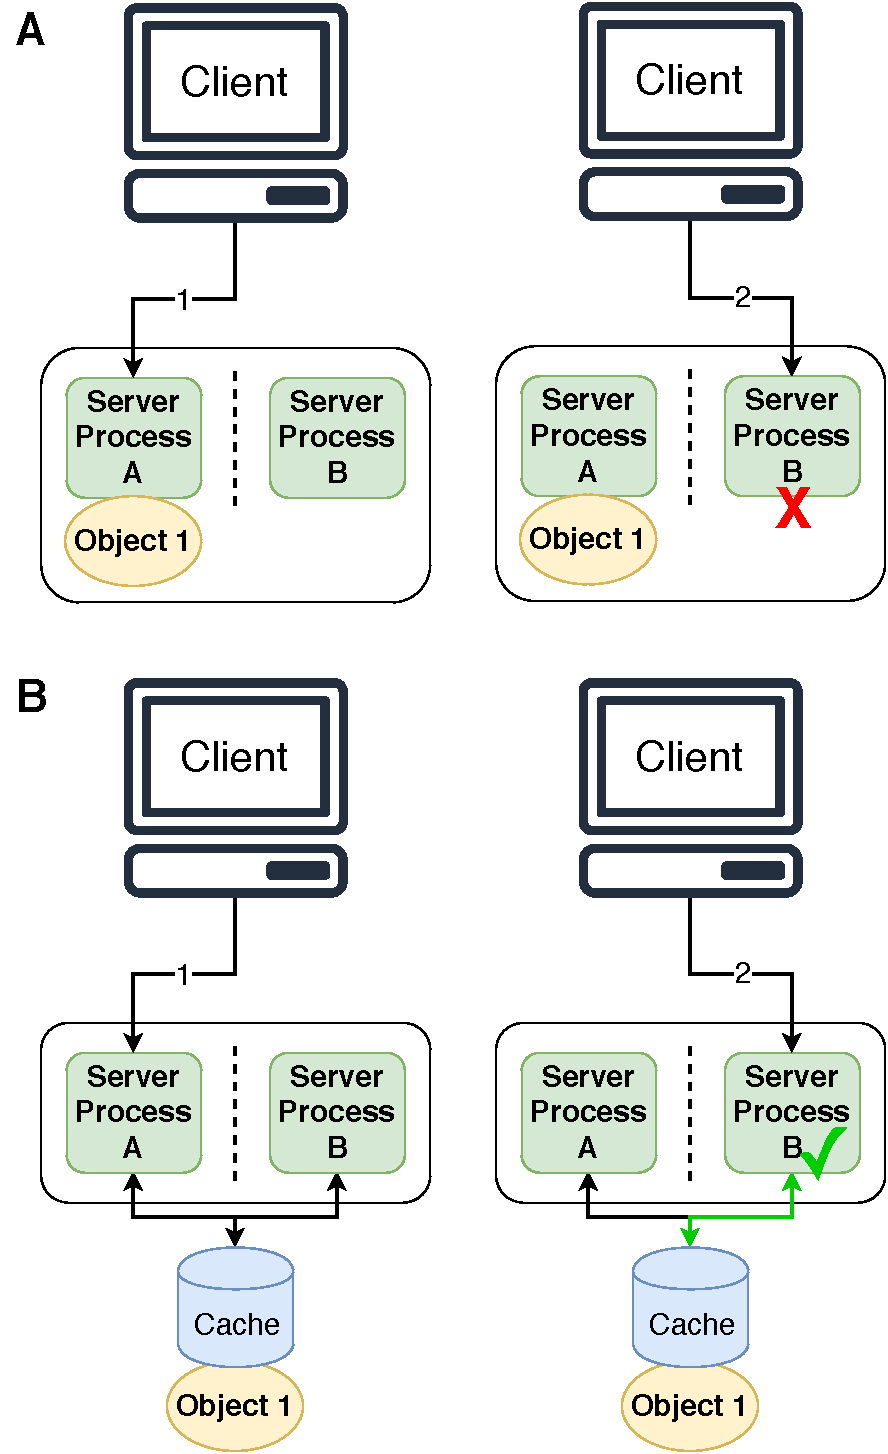
\includegraphics[width=0.50\textwidth]{media/Client-Processing.pdf}
	 \caption[Requests directed towards Python web endpoints are spread out across 
multiple processes and sharing data between these processes is 
difficult.]{\textbf{Requests directed towards Python web endpoints are spread 
out across multiple processes and sharing data between these processes is 
difficult.} (A) Processes cannot share in-memory objects directly due to 
operating system enforced process boundaries. (B) In order for data to be shared 
between request handling processes, it must be stored by a third central 
process, such as a cache or database.}
	 \label{fig:client-processing}
\end{figure}

\section{Application Programming Interface Endpoints} \label{endpoints}

Micromeda-Server provides several endpoints for supplying web clients with 
information about individual genome properties and information from uploaded 
Micromeda files. These endpoints were written using the Flask Python web 
framework \cite{grinberg2018flask} and are represented by \textbf{clean 
\gls{url}s} (see 
\href{http://en.wikipedia.org/wiki/Clean_URL}{en.wikipedia.org/wiki/Clean\_URL}) 
where some information that would normally be stored as \gls{http} GET 
parameters are stored in the \gls{url} path (Fig. \ref{fig:endpoint-url}). Flask 
was chosen due to its simplicity as compared to more comprehensive frameworks 
such as Django \cite{holovaty2009definitive}. The endpoints also follow a 
\gls{rest} architecture \cite{fielding2000representational} (see 
\href{http://en.wikipedia.org/wiki/Representational_state_transfer}{en.wikipedia.org/wiki/Representational\_state\_transfer}). 
These endpoints and their implementation are summarized in Table 
\ref{tab:endpoints}, Fig. \ref{endpoints}, Fig. \ref{fig:endpoint-url}, and 
detailed in subsections below.

\begin{figure}[!ht]
  \centering
	
\includegraphics[width=0.95\textwidth]{media/Coloured-Endpoint.pdf}
	 \caption[Micromeda-Server uses data held within URLs to figure out what 
information to return for a given HTTP request.]{\textbf{Micromeda-Server uses 
data held within \gls{url}s to figure out what information to return for a given 
\gls{http} request.} The example \gls{url} above is used to download a FASTA 
file containing the top proteins (\textit{i}.\textit{e}., those with the lowest \gls{eval} 
domains) that support GenProp0526 step one for dataset FXDABADS. The \gls{url} 
path variables are in blue and the \gls{http} GET parameters are in green. Note 
that the \gls{url} above is an example and does not point towards an active copy 
of Micromeda-Server or Micromeda-Client. Links to a demonstration of the client 
interface can be found in Section \ref{client-demo}.}
	 \label{fig:endpoint-url}
\end{figure}

\begin{longtable}{|p{1.6cm}|p{2.5cm}|p{1.4cm}|p{2.2cm}|p{2.2cm}|p{4cm}|}
\caption[Micromeda's server component provides web applications with five 
endpoints.]{Micromeda's server component provides web applications with five 
endpoints. By using the endpoints, these clients can request data about 
individual genome properties, upload Micromeda files, and request information 
about stored assignment databases.}
\label{tab:endpoints}\\

\hline
\textbf{Python Function Name} & \textbf{Endpoint URL} & \textbf{HTTP Request 
Types} & \textbf{URL Path Variables} & \textbf{GET Parameter Variables} & 
\textbf{Return Value} \\ \hline
\endfirsthead
%
\multicolumn{6}{c}%
{{\bfseries Table \thetable\ continued from previous page}} \\
\hline
\textbf{Python Function Name} & \textbf{Endpoint URL} & \textbf{HTTP Request 
Types} & \textbf{URL Path Variables} & \textbf{GET Parameter Variables} & 
\textbf{Return Value} \\ \hline
\endhead
%
upload & /upload & GET, POST & None & None & \gls{json} containing a dataset key 
that can be used by future \gls{api} requests to access information from the 
uploaded Micromeda file \\ \hline
get\_tree & /genome \_properties \_tree & GET & None & dataset\_key (optional) & 
\gls{json} tree representing all properties in the current Genome Properties 
database with each node annotated with a list of YES, NO, PARTIAL assignments 
for each organism in a dataset. \\ \hline
get\_single \_genome \_property \_info & /genome \_properties/ 
\textless{}string: property\_id\textgreater{} & GET & property\_id & None & 
\gls{json} containing information about a genome property such as a description 
of it and a list of equivalent records from other databases (\textit{e}.\textit{g}., \gls{kegg} 
\cite{kawashima2003kegg}, MetaCyc \cite{karp2002metacyc}) \\ \hline
get \_multiple \_genome \_property \_info & /genome \_properties & GET & None & 
None & \gls{json} array containing information about all genome properties in 
the database. Each property is given a description and a list of equivalent 
records from other databases (\textit{e}.\textit{g}., \gls{kegg}, MetaCyc) \\ \hline
get\_fasta & /fasta/ \textless{}string: property\_id\textgreater{}/ 
\textless{}int:step \_number\textgreater{} & GET & property\_id, step\_number & 
dataset\_key (optional), all (optional) & FASTA file containing either all or 
the top proteins (\textit{i}.\textit{e}., those with the lowest \gls{eval} domain annotations) 
supporting the existence of a given property step. A dataset key can be provided 
to specify a dataset. \\ \hline
\end{longtable}

\subsection{The Upload Endpoint} \label{endpoint-upload}

This \gls{api} endpoint accepts the client upload of a Micromeda file and 
returns a hexadecimal encoded \gls{uuid} key \cite{leach2005universally} (see 
\href{http://en.wikipedia.org/wiki/Universally_unique_identifier}{en.wikipedia.org/wiki/ 
Universally\_unique\_identifier}) to the client. After upload, the Micromeda 
file is parsed and transformed into a GenomePropertiesResultsWithMatches object. 
This object is then serialized to MessagePack using the object's 
\textbf{to\_msgpack} function (Table \ref{tab:genomepropertyresultswithmatches}) 
and the resulting binary is cached in Redis using the Redis Python library 
\cite{mccurdy_2019} (Fig. \ref{fig:micromeda-server-workflow}). During the 
previous process, a \gls{uuid}, to be used as a dataset key, is generated using 
Python's built in \gls{uuid} generation function \cite{PythonUUID}. This 
\gls{uuid} is used as the key for accessing the MessagePack serialization stored 
in the Redis cache (Fig. \ref{fig:micromeda-server-workflow}). Micromeda-Server 
returns the key to the client application in response to the file upload. The 
client can provide this key to other \gls{api} endpoints to receive data from 
the uploaded Micromeda file (Fig. \ref{fig:micromeda-server-workflow}). 

\subsection{The Get\_Tree Endpoint} \label{get-tree}

The \textbf{get\_tree} endpoint provides the client with a \gls{json} tree 
representing all properties and steps in Genome Properties database (Fig. 
\ref{fig:tree-json}). This tree represents parent-child relationships between 
properties. Step nodes are also attached to their parent genome property nodes 
and act as leaves (Fig. \ref{fig:tree-json}). Note that this endpoint returns a 
tree rather than a \gls{dag} (Fig. \ref{fig:tree-json}). In this tree, 
properties that would have had two parents in the Genome Properties \gls{dag} 
(Section \ref{genome-properties-overview}) are duplicated (Fig. 
\ref{fig:tree-json}). Each property and step node in the tree is annotated by a 
list of assignments of support (\textit{i}.\textit{e}., YES, NO, PARTIAL), one for each sample in 
a previously uploaded or default Micromeda file (Fig. \ref{fig:tree-json}). The 
\textbf{Get\_Tree} endpoint can take a \textbf{dataset\_key} \gls{http} GET 
parameter variable (Table \ref{tab:endpoints}). If a dataset key generated by 
the previous upload of a Micromeda file is assigned to this variable, then the 
assignments of support stored in the key's associated Micromeda file are 
returned. The dataset key is used to reconstitute a 
GenomePropertiesResultsWithMatches object, representing the uploaded Micromeda 
file, from the Redis cache. The GenomePropertiesResultsWithMatches object's 
\textbf{to\_json} method (Table \ref{tab:genomepropertyresultswithmatches}) is 
called to generate the above tree \gls{json}. This \gls{json} returned to the 
client by the endpoint. If no dataset\_key is provided to the endpoint, 
GenomePropertiesResultsWithMatches object of the default Micromeda is used to 
generate the tree \gls{json} using the same method.

\begin{figure}[!ht]
  \centering
	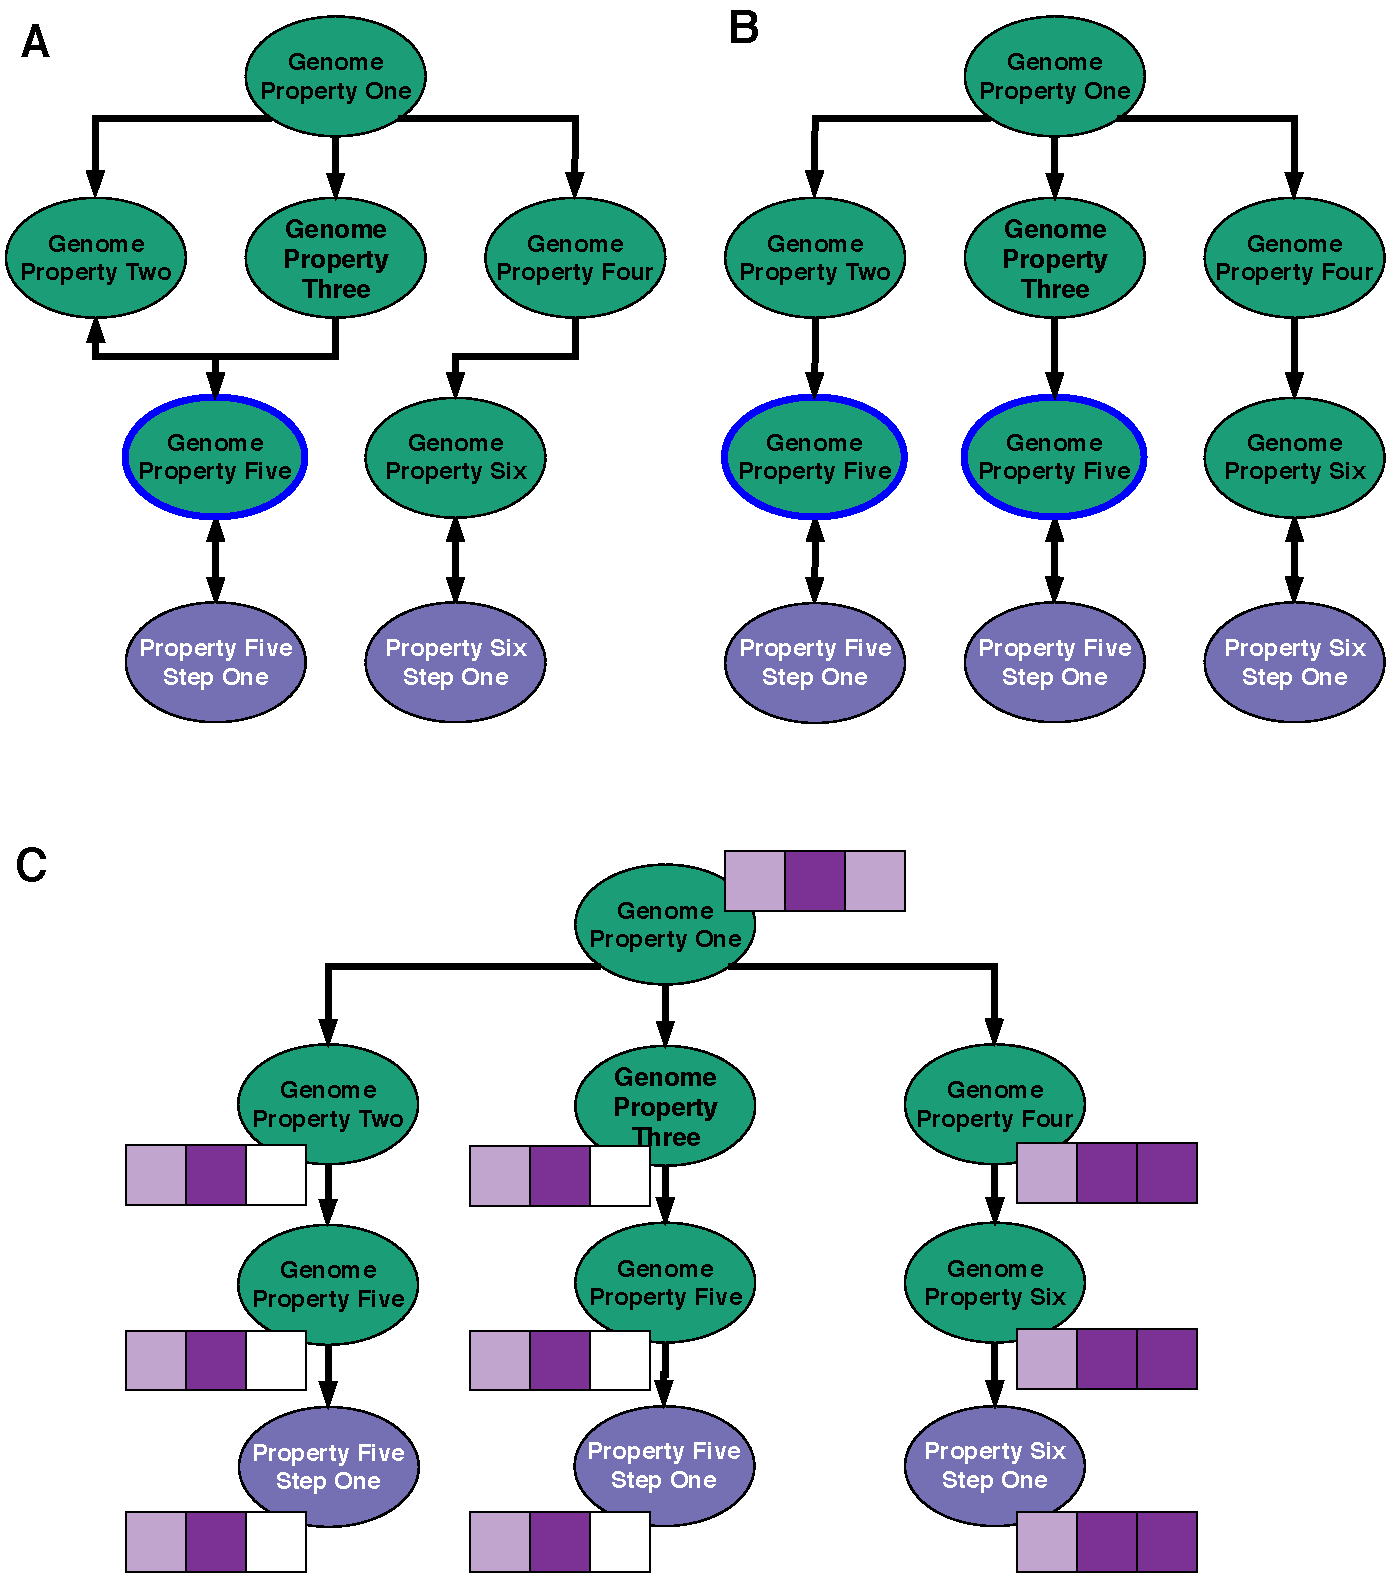
\includegraphics[width=0.70\textwidth]{media/Tree-JSON.pdf}
	 \caption[Micromeda-Server's Get\_Tree endpoint returns a Genome Property tree, 
not a DAG.]{\textbf{Micromeda-Server's Get\_Tree endpoint returns a Genome 
Property tree, not a \gls{dag}.} Unlike a \gls{dag} (A), a tree (B) cannot have 
branches that merge. Thus, the \gls{json} returned by the Get\_Treecan endpoint 
has some Genome Property nodes duplicated (B). In this JSON document, each node 
is tagged with a list of YES (Dark Purple), PARTIAL (Light Purple), and NO 
(White) assignments (C). Each assignment in this list belongs to a single 
organism in a dataset.}
	 \label{fig:tree-json}
\end{figure}

\subsection{The Get\_Single\_Genome\_Property\_Info Endpoint} 
\label{get-property-info-endpoint}

The \textbf{get\_single\_genome\_property\_info} endpoint takes a genome 
property identifier as a \gls{url} parameter (Table \ref{tab:endpoints}). This 
genome property identifier is used query for a matching GenomeProperty object 
(Section \ref{genome-property-class}), representing the property whose 
identifier is specified, from a global GenomePropertiesTree object (Section 
\ref{GenomePropertiesTree-Class}) created on Micromeda-Server's start up 
(Section \ref{server-workflow}). If found, this GenomeProperty object's 
\textbf{to\_json} method (Table \ref{tab:genome-property-object}) is called to 
create a \gls{json} document containing property information that is returned by 
the endpoint. This \gls{json} document includes the property name, property 
description, and a list of equivalent records from other databases (Table 
\ref{tab:genome-property-object}).

\subsection{The Get\_Multiple\_Genome\_Property\_Info Endpoint}

When the \textbf{get\_multiple\_genome\_property\_info} endpoint is called, the 
\textbf{to\_json} method (Table \ref{tab:genome-property-object}) is called on 
every GenomeProperty object (Section \ref{genome-property-class}), which is a 
child of the GenomePropertiesTree object (Section 
\ref{GenomePropertiesTree-Class}) created on Micromeda-Server start up. Each of 
the \gls{json} strings generated are placed into a list in a single larger 
\gls{json} document, which is then returned by the endpoint. 

\subsection{The Get\_Fasta Endpoint} \label{get-fasta-endpoint}

The \textbf{get\_gasta} endpoint is used to send the client a FASTA file 
containing protein sequences that support the existence of a property step 
across multiple organisms in a specific uploaded dataset. The \gls{url} path of 
requests to this endpoint includes the genome property identifier and step 
number of the property step required to generate a FASTA file. The FASTA file 
can either contain all proteins that support the existence of a property step or 
only those with the lowest \gls{eval} for the InterPro domain offering support 
for a given step. These proteins are known as the \textbf{``top"} hits. The 
contents of the returned file is controlled by the presence of a \gls{http} GET 
parameter called \textbf{all} (Fig. \ref{fig:endpoint-url}). If \textbf{all} is 
set to true, then a FASTA file containing all proteins that support a step is 
returned. Otherwise, a FASTA file containing only the lowest \gls{eval} proteins 
is returned. Like the Get\_Tree endpoint, this endpoint also accepts a 
\textbf{dataset\_key} \gls{http} GET parameter (Fig. \ref{fig:endpoint-url}). 
The value of this variable is used to reconstitute a 
GenomePropertiesResultsWithMatches object representing a previously uploaded 
Micromeda file (Fig. \ref{fig:micromeda-server-workflow}). This object's 
\textbf{write\_supporting\_proteins\_for\_step\_fasta} function (Table 
\ref{tab:genomepropertyresultswithmatches}) is used generate the FASTA file, 
which is sent to the client.

\section{Micromeda Server Performance} \label{micromeda-server-performance}

The performance of Micromeda's endpoints was tested using a Micromeda file 
generated from the protein sequences and InterProScan annotations of 
\textit{Chlorobium chlorochromatii} CaD3 (\gls{ncbitaxa}: 340177) and 
\textit{Pelodictyon luteolum} DSM 273 (\gls{ncbitaxa}:  319225). 
\textbf{Performance numbers for this section were recorded using Safari's 
(version 13; \href{http://apple.com/safari}{apple.com/safari}) Web Inspector.} 
When this file was sent to the \textbf{upload} endpoint of Micromeda-Server, it 
was parsed and added to the Redis cache in 11.3 s \textpm 2.0 s (\gls{n} = 3). 
The \textbf{get\_tree} endpoint could create a genome property tree from this 
cached Micromeda file in 9.4 s \textpm 4.0 s (\gls{n} = 3). The 
\textbf{get\_fasta} endpoint could generate a FASTA file with the top supporting 
proteins for GenProp0633 step number two in 33.0 ms \textpm 4.0 ms (\gls{n} = 
10). The property information \gls{json} file could be generated for GenProp0633 
by the \textbf{get\_single\_genome\_property\_info} endpoint in 7.0 ms \textpm 
2.0 ms (\gls{n} = 10). The \textbf{get\_multiple\_genome\_property\_info} can 
generated \gls{json} files for all properties in 23.0 ms \textpm 5.0 ms (\gls{n} 
= 10). The slow execution time of the \textbf{upload} and \textbf{get\_tree} 
endpoints was a result of latency in client applications. For example, there was 
a noticeable delay in the rendering of visualizations in Micromeda's client 
application. Thus the performance of these endpoints should be optimized and 
potential optimizations are discussed in Section 
\ref{micromeda-server-improvements}.

\section{Micromeda Server Deployments} \label{micromeda-server-deployments}

It is common to deploy web servers in different configurations depending on the 
expected request volume. Three deployment strategies of increasing size will be 
discussed below. 

\subsection{Development and Single User Deployment}

If a user wishes to install and run Micromeda-Server on their desktop or laptop 
and only needs to visualize one dataset at a time, then a very simplified 
deployment strategy can be used (Fig. \ref{fig:micromeda-small-deploy}). This 
deployment uses Flask's built in development \gls{http} server to respond to 
requests. The server is activated when Micromeda-Server's Python script is run 
directly from a \gls{cli}. This single-user deployment is slow and can only 
handle single requests from single clients. In this configuration, Redis is not 
required, and users must tell Micromeda-Server to use their dataset (\textit{i}.\textit{e}., a 
Micromeda file) as its default (Fig. \ref{fig:micromeda-small-deploy}). The 
upload endpoint is also turned off. This deployment method is similar to the one 
used by Anvio's \gls{mags} visualization and refinement server 
\cite{eren2015anvi}. The single-user deployment configuration is also useful for 
developers who want to test newly developed features or bug fixes.

\begin{figure}[!ht]
  \centering
	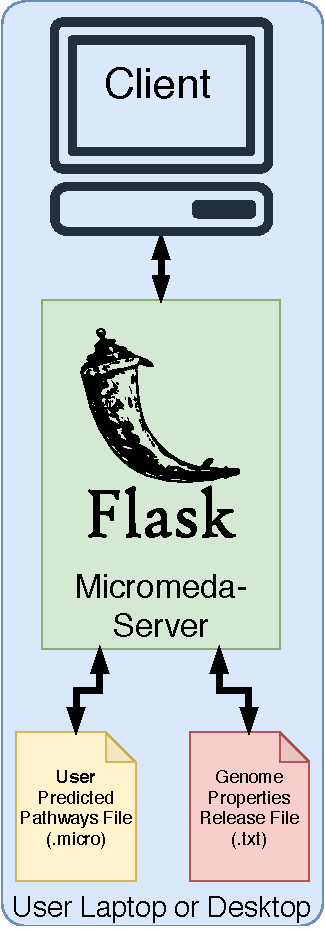
\includegraphics[width=0.25\textwidth]{media/micromeda-simple-deployment.pdf}
	 \caption[Micromeda-Server can be deployed in a manner that only visualizes 
Micromeda files stored on the server that hosts it.]{\textbf{Micromeda-Server 
can be deployed in a manner that only visualizes Micromeda files stored on the 
server that hosts it.} In this deployment style, Micromed-Server uses Flask's 
builtin \gls{http} server, a genomeProperties.txt file, and the server-side 
Micromeda file. This deployment style is excellent for development use or 
deployment to individual user laptops and desktops. However, this deployment 
style encounters problems when used by multiple users because only a single copy 
of the client Python is run at a time.}
	 \label{fig:micromeda-small-deploy}
\end{figure}

\subsection{Single Server Deployment} \label{single-server-micromeda-deployment}

If a user requires Micromeda-Server to handle multiple users simultaneously, 
such as would be the case if it was installed on a server computer system, a 
larger deployment must be used (Fig. \ref{fig:micromeda-medium-deploy}). This 
deployment type adds additional software layers that increase Micromeda-Server's 
scalability. As discussed in previous sections, multiple copies of 
Micromeda-Server's Python code must be run simultaneously to handle multiple 
client requests. This technique is done by putting the Micromeda-Server under 
the command of a master \gls{http} server that can route traffic to multiple 
copies of the code in separate processes (Fig. 
\ref{fig:micromeda-medium-deploy}). Such master \gls{http} servers include the 
Apache \cite{fielding1997apache} and Nginx \cite{reese2008nginx} \gls{http} 
servers. This master server handles the parsing of \gls{http} requests. In 
addition to the master server, a middleware component, such as uWSGI 
\cite{2019uwsgi} or gunicorn \cite{chesneau_2018}, must also be used. Redis is 
used to cache GenomePropertiesResultsWithMatches objects between requests in 
this deployment type. All components of the above server are deployed on the 
same server computer system (Fig. \ref{fig:micromeda-medium-deploy}).

\begin{figure}[!ht]
  \centering
	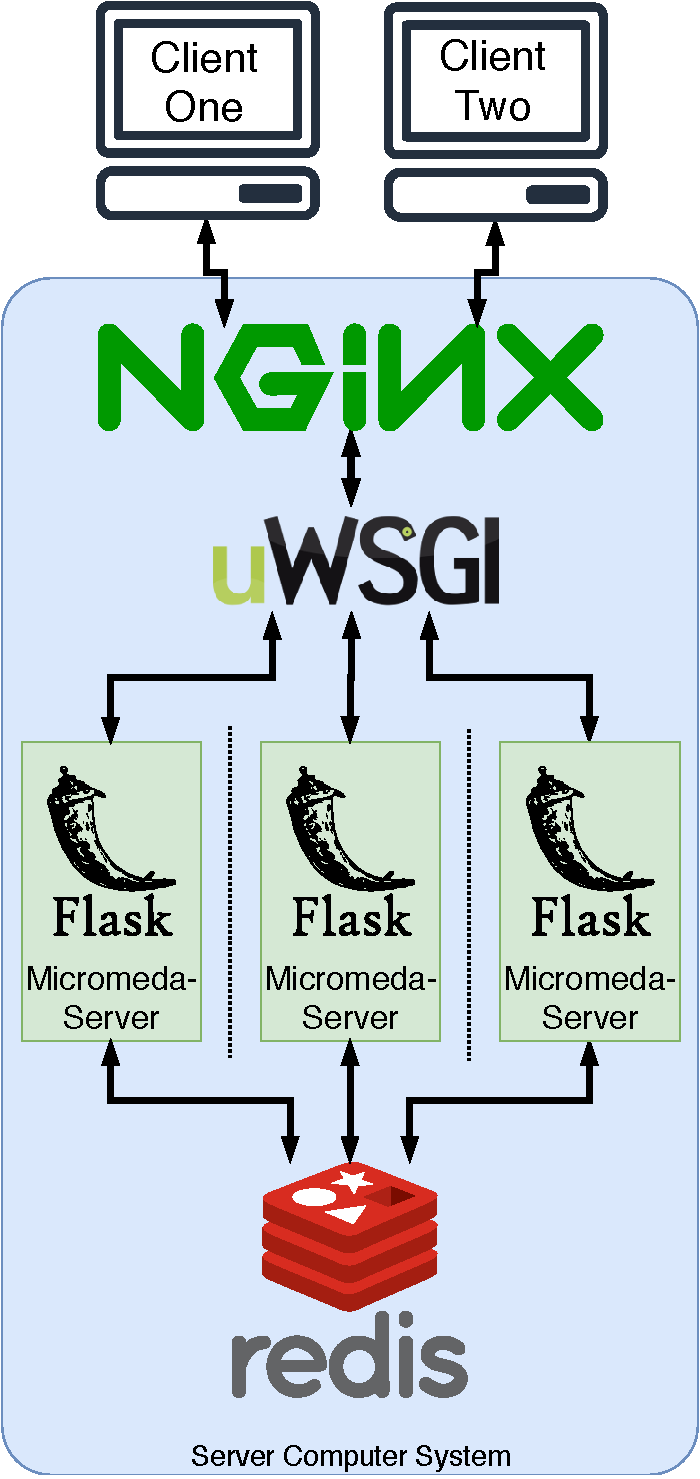
\includegraphics[width=0.35\textwidth]{media/micromeda-medium-deployment.pdf}
	 \caption[When deployed to handle the traffic of multiple clients, 
Micromed-Server must be supported by multiple other types of 
software.]{\textbf{When deployed to handle the traffic of multiple clients, 
Micromed-Server must be supported by multiple other types of software.} In this 
deployment style, multiple copies of its Python code are run simultaneously to 
handle multiple clients. Redis is used to provide shared data between these 
processes. A uWSGI middleware component is used to connect these copies to a 
high performance \gls{http} server, such as Nginx, that can handle high web 
traffic volumes. The genomeProperties.txt files and default Micromeda files are 
still used in this deployment style but were omitted from the diagram for 
simplicity.}
	 \label{fig:micromeda-medium-deploy}
\end{figure}

\subsection{Multiple Server Deployment} 
\label{multi-server-micromeda-deployment}

For a large number of simultaneous users, Micromeda-Server may need to be scaled 
horizontally to multiple servers (Fig. \ref{fig:micromeda-large-deploy}). This 
scaling is done by placing a load balancer 
(\href{http://en.wikipedia.org/wiki/Load_balancing_(computing)}{en.wikipedia.org/wiki/Load\_balancing\_(computing)}) 
out front of multiple copies of the previous deployment running on separate 
server computer systems (Fig. \ref{fig:micromeda-large-deploy}). Redis can also 
be run on a separate server computer system or computing cluster (Fig. 
\ref{fig:micromeda-large-deploy}). Such multiple server deployment strategies 
can be scaled horizontally by adding new server computer systems to the 
deployment (Fig. \ref{fig:micromeda-large-deploy}). These new server computer 
systems can handle increases in request volume.

\begin{figure}[!ht]
  \centering
	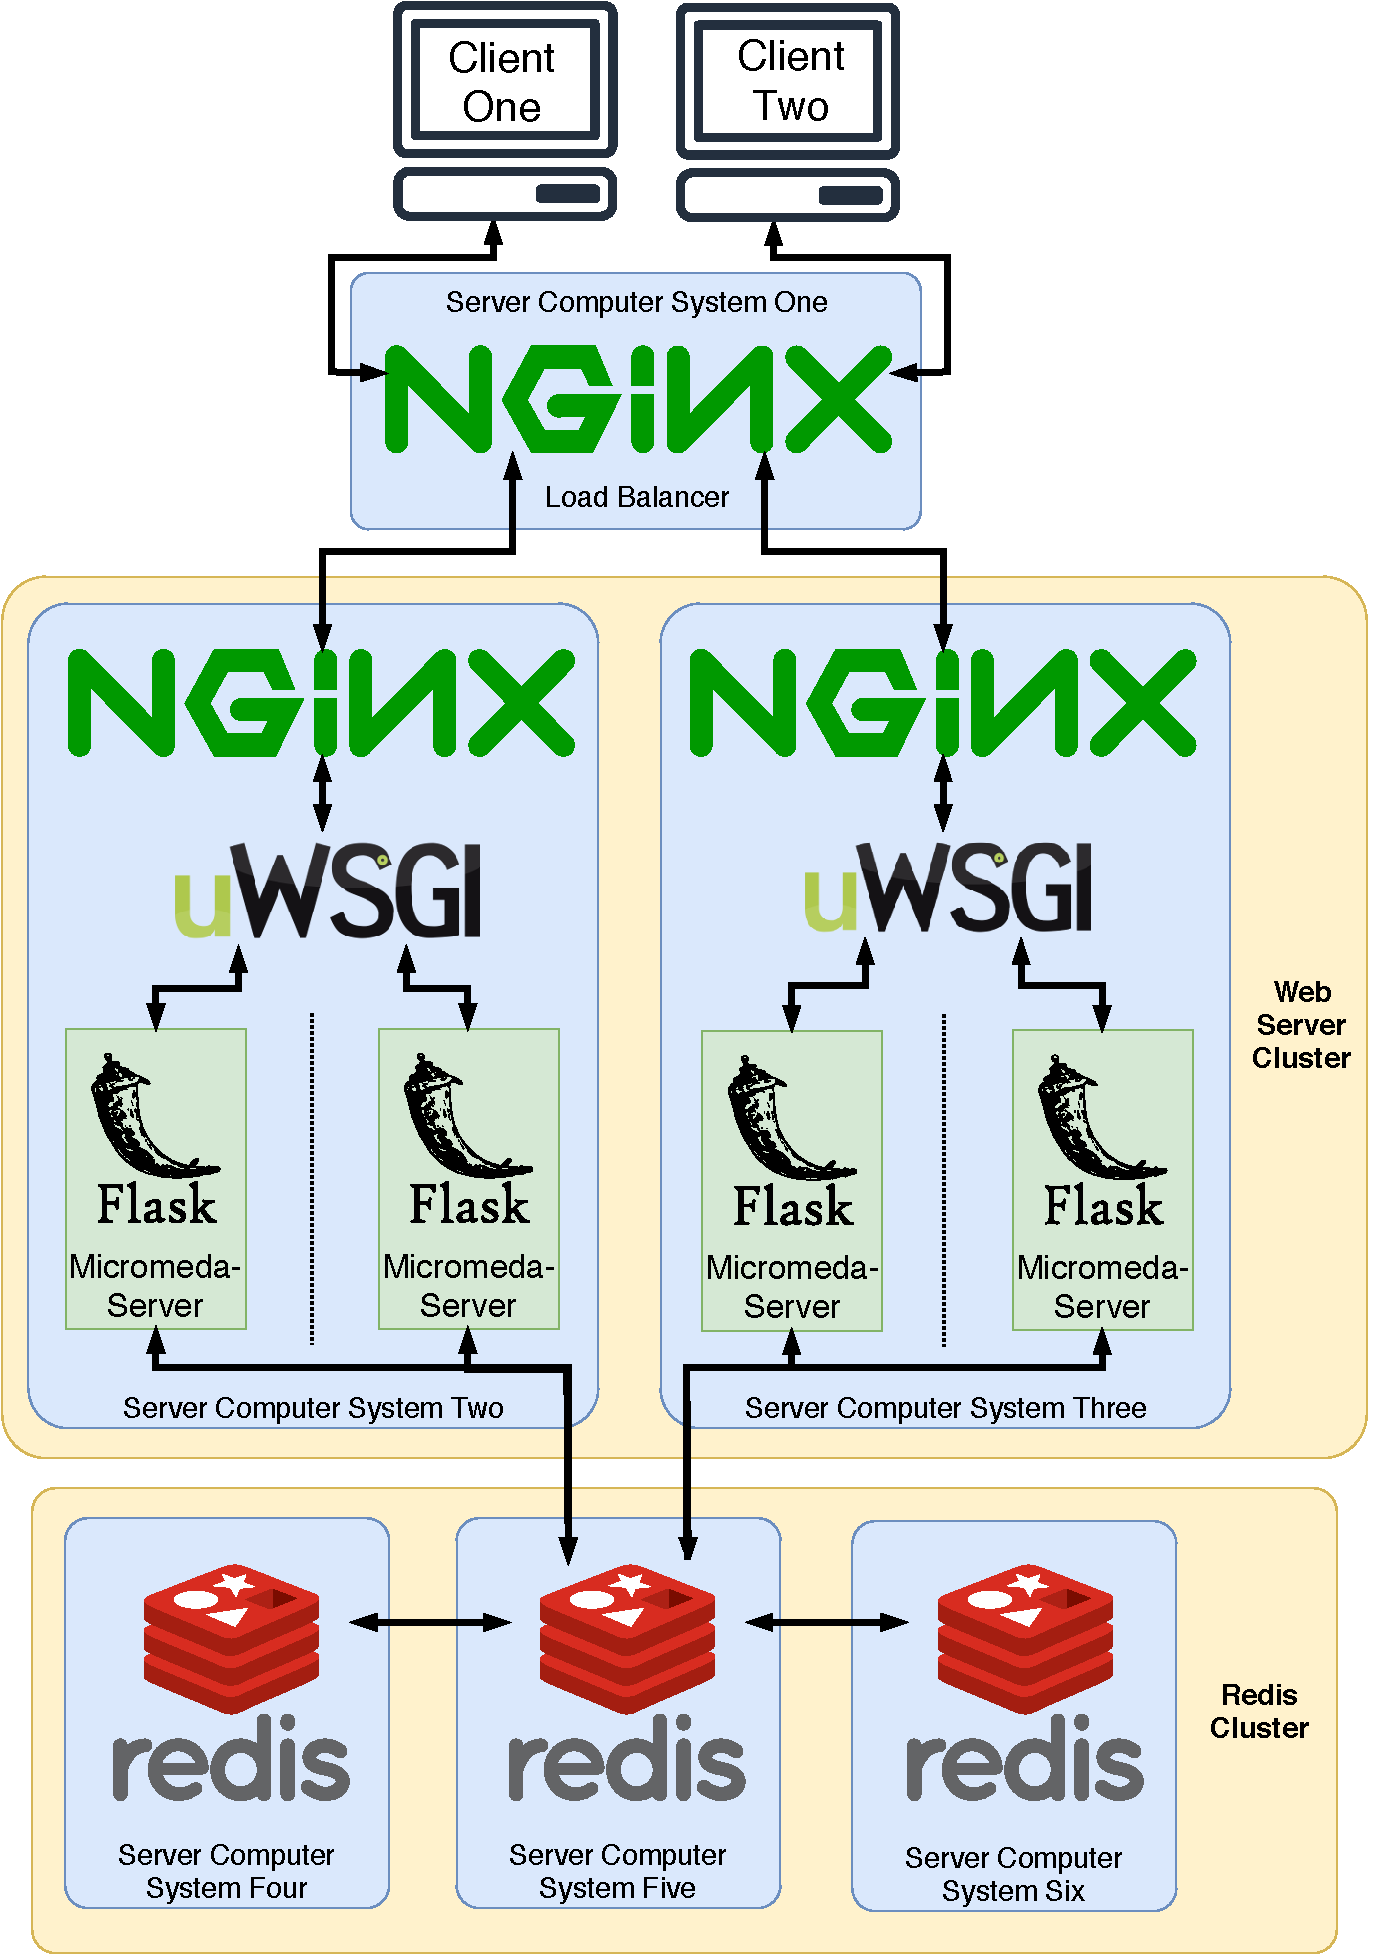
\includegraphics[width=0.60\textwidth]{media/micromeda-heavy-deployment.pdf}
	 \caption[When Micromeda is required to scale to handle hundreds or thousands 
of simultaneous users, its workload must be spread out across multiple caching 
and web server computer systems.]{\textbf{When Micromeda is required to scale to 
handle hundreds or thousands of simultaneous users, its workload must be spread 
out across multiple caching and web server computer systems.} Each node in the 
webserver cluster runs additional copies of Micromeda-Server and supporting 
software. The performance of such deployments can be increased by adding 
hardware to either of the caching or web server clusters.  A copy of the 
genomeProperties.txt file and default Micromeda file would be stored in each web 
server and have been omitted from the diagram for simplicity.}
	 \label{fig:micromeda-large-deploy}
\end{figure}

\subsection{Cloud Platform As A Service (PaaS) Deployment}

Various cloud computing corporations have developed \gls{paas} 
\cite{lawton2008developing} products (see 
\href{http://en.wikipedia.org/wiki/Platform_as_a_service}{en.wikipedia.org/wiki/Platform\_as\_a\_service}) 
that help users scale Python web applications without having to spend the time 
setting up complex multiple server deployments as discussed above. These 
\gls{paas}, such as Google App Engine 
(\href{http://cloud.google.com/appengine}{cloud.google.com/ appengine}) or 
Heroku (\href{http://heroku.com}{heroku.com}), provide the simplicity of a 
single user deployment with the scalability of multiple server deployments. They 
do this by only requiring the developers to upload their Flask Python code and 
then automate the rest of the deployment process. For example, load balancers 
and multiple copies of request handling processes are spun up by such platforms 
automatically. Such platforms perform these tasks in the background and 
invisibly to the developer who uploaded the code.

\section{Future Improvements} \label{micromeda-server-improvements}

Micromeda-Server currently provides endpoints for all the information needed by 
Micromeda's web-based visualization client. However, in addition to the existing 
endpoints, new endpoints could be made that would provide new data for future 
versions of this client, allowing it to have expanded functionality. Performance 
optimizations for the existing endpoints could also be made, which could reduce 
latency in the client's \gls{ui} by reducing the time spent waiting for 
responses from Micromeda-Server. Improvements to Micromeda-Server's existing 
endpoints and a potential new endpoint are discussed below.

\subsection{Improving Performance of the Upload Endpoint}

The \textbf{upload} endpoint takes a Micromeda file and saves its contents to a 
Redis cache. This endpoint was shown to have poor performance (see Section 
\ref{micromeda-server-performance}) and should be optimized to make it respond 
faster. Most of the performance problems with this endpoint can be attributed to 
the performance of parsing Micromeda files into 
GenomePropertiesResultsWithMatches objects using the 
\textbf{load\_assignment\_caches\_from\_database \\ \_with\_matches} function of 
Pygenprop's results module. The performance of this function was also weak (see 
Subsection \ref{micromeda-file-performance}). Performance improvements to this 
function are discussed in detail in Subsection 
\ref{improving-pygenprop-performance}. The performance optimizations recommended 
in that section should be adopted and will drastically improve the performance 
of the upload endpoint.

\subsection{Improving Performance of the Get\_Tree Endpoint and Building 
Endpoints for Returning Property and Step Assignments} 
\label{assignment-endpoints}

The \textbf{get\_tree} endpoint sends \gls{json} to the client that contains 
both property tree and assignment data. This \gls{json} is generated by calling 
a GenomePropertiesResultsWithMatches object's \textbf{to\_json} method. This 
method is known to have speed issues (see Subsection \ref{matches-performance} 
and Section \ref{micromeda-server-performance}) due to the method having to 
insert assignments into the \gls{json} tree one at a time, rather than in batch. 
This speed issue could be addressed by reconfiguring Micromeda-Sever's 
\textbf{get\_tree} endpoint to no longer output a tree annotated by property 
assignments. Instead, new endpoints could be built that return step and property 
assignments separately (Fig. \ref{fig:new_endpoints}). New methods of 
GenomePropertiesResultsWithMatches objects would have to be developed to 
generate \gls{json} for these new endpoints (Section 
\ref{improving-pygenprop-performance}). The code for generating the property 
tree \gls{json} could be moved to the GenomePropertiesTree class (Fig. 
\ref{fig:new_endpoints}).

Caching the \gls{json} generated by endpoints in Redis could also improve their 
performance. On subsequent \gls{api} calls, the cached data could be recalled 
from Redis and immediately returned to the client instead of being regenerated 
with every \gls{api} call. For example, only having to generate a property tree 
once procedurally would significantly improve endpoint performance.

\begin{figure}[!ht]
  \centering
	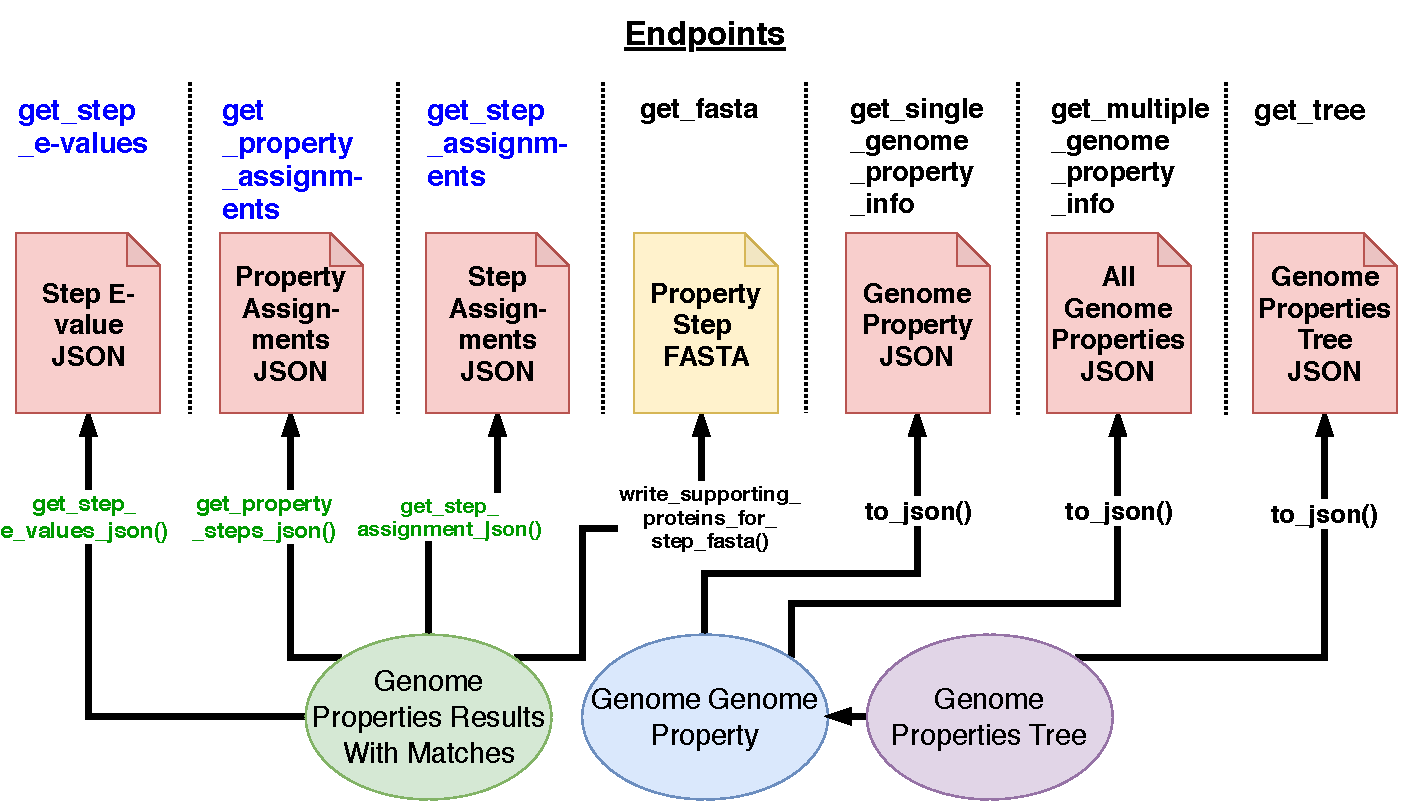
\includegraphics[width=0.8\textwidth]{media/micromeda-server-new-endpoints.pdf}
	 \caption[Future versions of Micromeda-Server could have new endpoints that 
allow for expanded functionality.]{\textbf{Future versions of Micromeda-Server 
could have new endpoints that allow for expanded functionality.} These endpoints 
would return step assignments, step supporting information, and property 
assignments (blue). They would be supported by new \gls{json} generating methods 
of GenomePropertiesResultsWithMatches objects (green).}
	 \label{fig:new_endpoints}
\end{figure}

\subsection{Creation of an Endpoint for Returning Domain Annotation Supporting 
Property Steps} \label{e-value-endpoint}

Micromeda files not only contain property and step assignments for a set of 
organisms but also contain additional information such as domain annotations and 
proteins sequences that support the existence of property steps. 
Micromeda-Server currently provides an endpoint for accessing protein sequences 
that support steps (see Subsection \ref{get-fasta-endpoint}). However, there are 
no endpoints for accessing the stored InterProScan annotations of these 
proteins. Specifically, these annotations contain \gls{eval} scores representing 
how closely the domain in the protein matches to a model of a representative 
domain in a protein database (see Section \ref{InterProDatabases}). The 
\gls{eval} scores for these domains may be useful for client visualizations that 
compare not only the presence and absence of proteins that support property 
steps but also compare how close these matches are to existing domain models. 
Thus, it may be useful to create a new endpoint that returns domain annotation 
\gls{eval} scores for domains that support property steps (Fig. 
\ref{fig:new_endpoints}). This endpoint could generated its data from the 
\textbf{step\_matches} DataFrame of reconstituted 
GenomePropertiesResultsWithMatches objects.

\section{Summary} \label{server-summary}

The creation of web server \gls{api}'s for accessing information about 
biochemical pathways, and even the precalculated presence and absence of these 
pathways across organisms, is quite common 
\cite{wu2006kobas,moriya2010pathpred,pireddu2006path,vallenet2009microscope,aziz2008rast,takami2016automated,moriya2007kaas,chou2009fmm}. 
Indeed, such web \gls{api}s have been developed by both the creators of 
\gls{kegg} \cite{kawashima2003kegg} and MetaCyc \cite{karp2013data}, not only 
for their web client applications but also for academic use. A web server has 
also been built for Genome Properties database website 
\cite{richardson2018genome} that is hosted by the \gls{ebi}. However, its 
\gls{api} is not publicly available and is only designed to support the Genome 
Properties website. The \gls{kegg}, MetaCyc, and Genome Properties website all 
contain precalculated pathway annotations for sets of reference organisms 
\cite{kanehisa2000kegg,karp2002metacyc,karp2013data}. However, its \gls{api} is 
not publicly available and is only designed to support the Genome Properties 
website. The \gls{kegg}, MetaCyc, and Genome Properties website all contain 
precalculated pathway annotations for sets of reference organisms 
\cite{kanehisa2000kegg,karp2002metacyc,karp2013data}. Many pathway annotation 
web sites such as \gls{fmm} \cite{chou2009fmm}, \gls{kaas} \cite{moriya2007kaas} 
and \gls{maple} \cite{takami2016automated} can pathway annotate user-supplied 
genomes uploaded in FASTA format \cite{pearson19905}. Such annotation servers 
are complex to build and host due to the relative computational complexity of 
scanning for genes that support the existence of pathway steps. In contrast, the 
Genome Properties website allows for the upload of user-created InterProScan 
annotation files. The creation of such annotations files pushes the most 
computationally complex part of the Genome Properties pipeline, domain 
annotation, off onto end-users \cite{richardson2018genome}. As discussed in 
Subsection \ref{why-micromeda-files}, Micromeda-Server follows a similar 
approach. However, unlike the Genome Properties website, Micromeda-Server takes 
the upload of Micromeda files. The use of Micromeda files provides a unique 
advantage to Micromeda-Server, in contrast to almost all other annotation 
servers, because it allows users to download information about supporting 
proteins and domain annotations if such an endpoint was created and used in 
pathway determination. Micromeda files also allow the upload of datasets 
consisting of pathway annotations from multiple genomes simultaneously, unlike 
other pathway servers, which often require uploading genomes or InterProScan 
annotations for organisms one at a time. With the avoidance of computationally 
complex annotation steps and a variety of horizontally scalable deployment 
options, Micromeda-Server should provide a reliable and sustainable \gls{api} 
for Micromeda's client application.
